\subsection{AES encryption round}

AES Encryption rounds consist of four transformations explained in previous sections. A circuit that can be used to implement a round is presented in figure \ref{fig:aes-round}. It is designed so that it can be used for all rounds - rounds 1 to 13 use \textit{block out} output, and last round uses \textit{last block out} output.

\begin{figure}[!H]
\centering
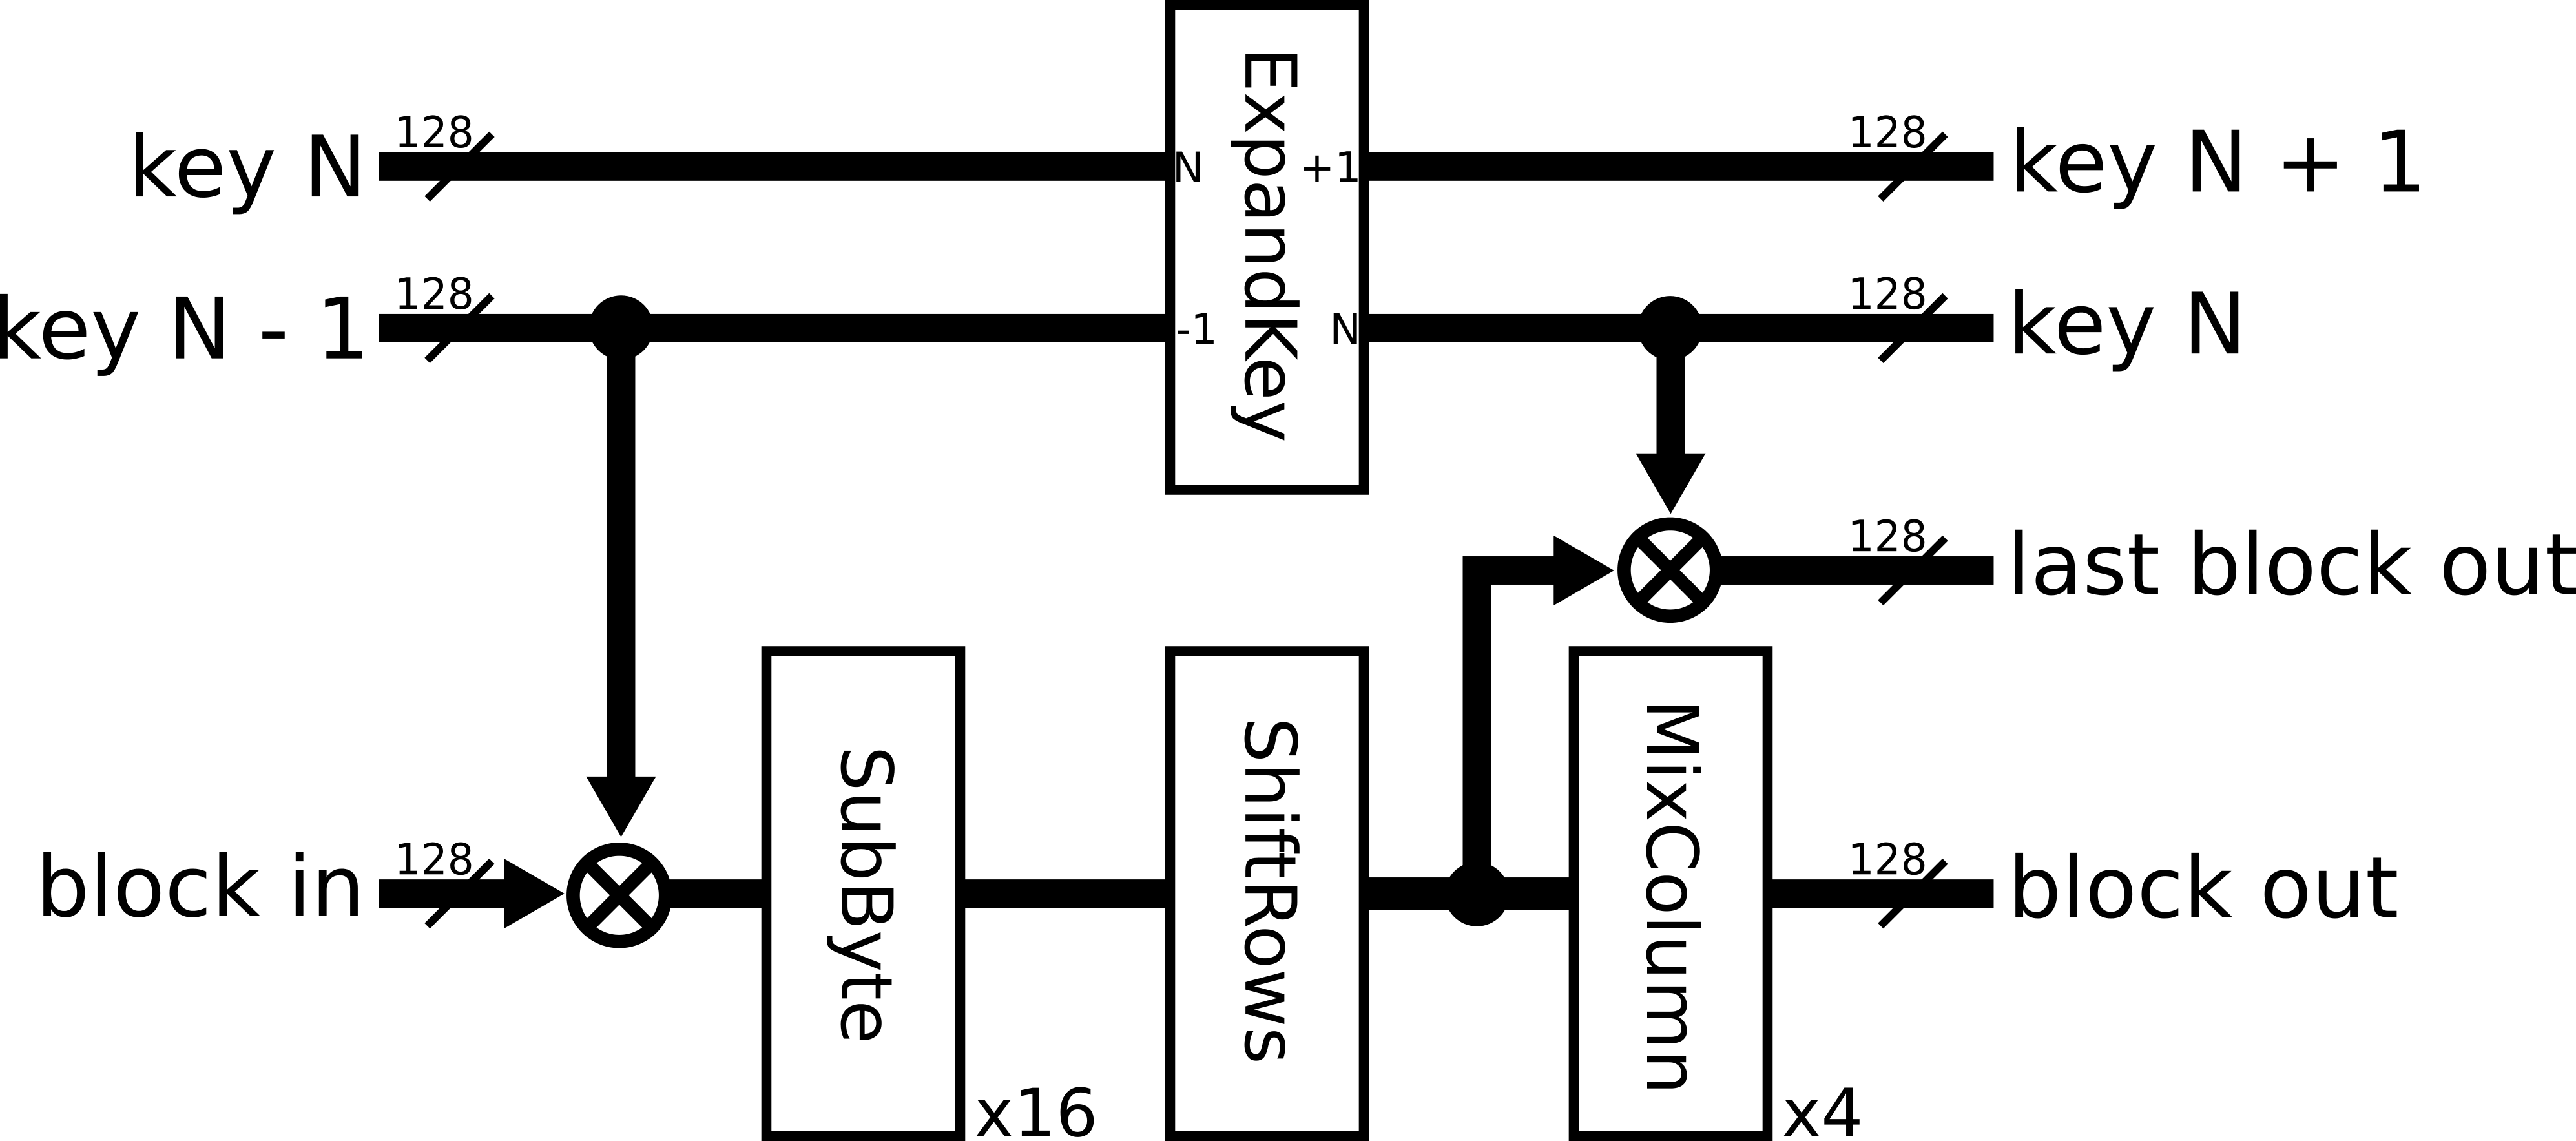
\includegraphics[scale=4]{aes-round}
\caption{AES round circuit}
\label{fig:aes-round}
\end{figure}

256-bit version of AES encryption algorithm, which is analysed here, has 14 rounds. Rounds 1 to 13 are the same and use all four transformations (fig. \ref{fig:aes-round}). Last round is different from other rounds in that it applies AddRoundKey transformation twice, and does not use MixColumns transformation.

